\chapter{Introduction} \label{chapt:Introduction}

In a machine learning application, a change in the data distribution is known as concept drift. Adapting to concept drift is one of the core problems in data stream learning \cite{big_data}.
Over the last few decades, considerable research has been dedicated to detecting and adapting to concept drift \cite{gama_survey}\cite{barros_comparison}. Because concept drift is such a broad category of phenomenon, this research has necessarily had to focus on a specific formulation of concept drift. The most common formulation is roughly
\begin{displayquote}
  At regular time intervals, new instances become available. A model must predict the label corresponding to each new instance. Immediately after the prediction has been made the true label becomes available. The learner then incrementally updates the model based on the new instance-label pair in an online manner.
\end{displayquote}
We will call this the {\bf standard formulation of the concept drift problem}, or simply the standard formulation. %A common variant of the standard formulation is that instances and labels become available in batches rather than individually. Practically, this often makes little difference. 

The standard formulation is attractive from an academic perspective. It is simple and covers a wide class of problems. It is easily rendered in synthetic benchmark datasets against which progress in the field can be measured. It can be naturally expressed in formal mathematics, so is easily tractable to theoretical study.

There are broadly two approaches to handling concept drift. ``Blind" approaches do not explicitly model drift, instead allowing the model to gradually adapt to the new environment. ``Informed" approaches, instead employ {\bf drift detectors} to explicitly detect when concept drift has occurred so that the model can be retrained \cite{gama_survey}. Blind approaches are often inadequate, as it can take too long for the model to adapt to the new environment. Informed approaches work roughly as follows:
\begin{displayquote}
  The drift detector monitors some performance metrics of the model. When it detects a degradation in performance, it infers that the model no longer reflects the current data distribution, and signals that concept drift has occurred. It then retrains the model using data which arrived after the drift was detected.
\end{displayquote}
We will call this the {\bf standard approach to concept drift adaptation}, and it is illustrated in Figure \ref{fig:standard_adaptation}.

\begin{figure}
    \centering
    
    % Define block styles
    \tikzstyle{decision} = [diamond, draw, fill=blue!20, 
        text width=4.5em, text badly centered, node distance=3cm, inner sep=0pt]
    \tikzstyle{block} = [rectangle, draw, fill=blue!20, 
        text width=5em, text centered, rounded corners, minimum height=4em]
    \tikzstyle{line} = [draw, -latex']
    \tikzstyle{cloud} = [draw, ellipse,fill=red!20, node distance=3cm,
        minimum height=2em]
    
    % Define block styles
    \begin{tikzpicture}[node distance = 2cm, auto]
        % Place nodes
        \node (start) {};
        \node [block, right of=start, node distance=3cm] (model) {Model};
        \node [block, right of=model, node distance=6cm] (detector) {Detector};
        \node [right of=model, distance=3cm] (mid) {};
        \node [cloud, below right of=model, align=center, node distance=4cm] (action) {retrain};
        % Draw edges
        \path [line] (start) -- node {data}(model);
        \path [line] (model) -- node {error rate}(detector);
        \path [line] (detector) |- node {drift detected} (action) -| (model);
        % \path [line] (action) ;
    \end{tikzpicture}
    \caption{Informed approach to concept drift adaptation.}
    \label{fig:standard_adaptation}
\end{figure}

\section{Motivation}

In many applications the standard formulation of the concept drift problem diverges from reality in important ways. In this thesis we explore some algorithms which help bridge the gap between academic concept drift detection and practical data science applications. %In some cases this may only mean that existing drift detectors are theoretically inappropriate, but practically serviceable. In other cases it may be a fatal flaw that renders drift detectors unusable.

We are motivated by a concrete problem from medical data science. We will return to this motivating example for illustration throughout the thesis. The problem is as follows.
\begin{displayquote}
  When a patient is referred to a medical facility, the referral is documented with free text and structured data, containing such information as condition, comorbidities, and demographics. From this data a clinician will make a decision about how urgently the patient needs to be addressed, and assign the patient a triage priority label. Some examples of triaging manuals are publicly available \cite{aus_triage}\cite{UK_mental_triage}\cite{musculoskeletal_services}.

  Referral documents are often electronic, reflecting a broad trend of medical facilities switching from paper documents to electronic health records (EHR)~\cite{ehr_adoption}. These electronic documents present an opportunity~\cite{ehr_opportunities}: supervised learning can be used to train a model which predicts triage labels for referral documents. This model can then be incorporated into a decision support system to help clinicians make more efficient and systematic triage decisions.

  An obvious benefit of such a support system is helping timely triaging of referrals. Automatic support system triage can provide a first pass on referrals, which can then be manually reviewed by clinicians. Another area in which this decision support system is expected to benefit public health is by countering potential bias in the healthcare system \cite{pdh}.

  Staff, resources, policy, and medical best practices evolve over time, and the decision support system must be able to detect and adapt to these changes. For instance, suppose a condition is discovered to be particularly dangerous for some demographic. Clinicians will likely increase the average priority of patients with the condition in this demographic. A decision support system must be able to promptly detect that such a change has occurred, and trigger appropriate actions for the model to be corrected. That is, a decision support system must be sensitive to {\it concept drift}.

  Within the medical context, a high degree of reliability is required. When concept drift is detected, a human expert is required to oversee and assist in the retraining of the model, as shown in Figure \ref{fig:referrals_triage}. When a GP makes a referral, the electronic referral document is sent to the model, a clinician, and a drift detector. The model predicts the triage label of the referral, and this prediction is sent to both the clinician, for decision support, and the drift detector. When the clinician decides on an ``official" triage label, this is also sent to the drift detector. The detector monitors the incoming referral documents, predictions, and labels for signs of concept drift. If drift is detected, a data scientist is alerted. The data scientist inspects the output of the drift detector, and the distribution of the data stream, and decides if the model is still fit for purpose (FFP). If not, the data scientist may decide to retrain the model, or recall the model if its performance cannot be recovered to an acceptable level.

  If the model is to be retrained, the data scientist must decide what data can be included in the new training set. For example, in the previous scenario, the model should be retrained on the full corpus of data, minus the referral documents of patients from the demographic group with the condition from before the priority change. The drift detector should help the data scientist figure out which data to use in retraining.
\end{displayquote}

\begin{figure}
    \centering
    \tikzstyle{block} = [rectangle, draw, 
        text width=5em, text centered, rounded corners, minimum height=6em] % fill=blue!20, 
    \tikzstyle{line} = [draw, -latex']
    \tikzstyle{cloud} = [draw, ellipse,fill=yellow!20, node distance=3cm,
        minimum height=3em]
    
    \begin{tikzpicture}[node distance = 3cm, auto]
        % Place nodes
        \node [block] (gp) {
\includegraphics[width=1cm]{images/referrals_triage/gp.png}\\GP};
        \node [cloud, right of=gp] (referral) {Referral};
        \node [cloud, above right of=referral, align=center] (support) {Decision\\support};
        \node [block, above of=support] (model) {
\includegraphics[width=1cm]{images/referrals_triage/model.png}\\Model};
        \node [block, below of=support, node distance=5cm] (clinician) {
\includegraphics[width=1cm]{images/referrals_triage/clinician.png}\\Clinician};
        \node [cloud, right of=clinician, node distance=4cm, align=center] (label) {Triage\\label};
        \node [cloud, right of=model, node distance=4cm] (prediction) {Prediction};
        \node [block, right of=referral, node distance=6cm] (detector) {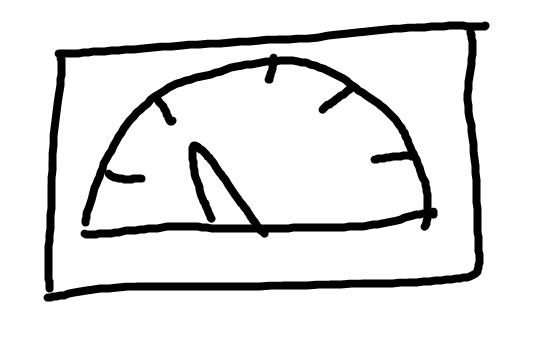
\includegraphics[width=1cm]{images/referrals_triage/detector.png}\\Detector};
        \node [cloud, above of=model] (retrain) {Retrain};
        \node [cloud, right of=detector, align=center] (detection) {Drift\\detection};
        \node [block, above of=retrain] (ds) {
\includegraphics[width=1cm]{images/referrals_triage/datascientist.png}\\Data scientist};
        % Draw edges
        \path [line] (gp) -- (referral) -- (detector);
        \path [line] (referral) |- (clinician);
        \path [line] (clinician) -- (label) -- (detector);
        \path [line] (referral) |- (model);
        % \path [line] (referral) -- (detector);
        \path [line] (model) -- (prediction) -- (detector);
        \path [line] (detector) -- (detection) |- (ds);
        \path [line] (ds) -- (retrain);
        \path [line] (retrain) -- (model);
        \path [line, dashed] (model) -- (support) -- (clinician);
    \end{tikzpicture}
    \caption{The proposed method for handling concept drift in GP referrals triage.}
    \label{fig:referrals_triage}
\end{figure}

This setting diverges from the standard concept drift problem formulation in that there may be an arbitrarily long delays between new instances arriving and correct labels becoming available. Furthermore, the labels may become available in a different order to instances.

Also, unlike in the standard approach where the detector automatically retrains the model when drift is detected, in the GP referrals context, a human in the loop oversees and assists in model retraining. 

How should a concept drift detector be designed to meet these challenges?

\section{Problem Statement}


% In order to make an informed decision about what action to take, the data scientist will want to know:
% \begin{itemize}
%   \item Has the distribution of referrals changed? And if so, does this require model retraining or recall? Can this be detected before all the labels have arrived, which could take arbitrarily long?
%   \item Will retraining the model on more recent data actually improve its performance? Or is performance irreparably degraded under the new distribution because the referral tasks have become intrinsically more difficult?
%   \item How severe was the concept drift and how long ago did it occur? Can the uncertainty on these questions be quantified?
% \end{itemize}
% Existing drift detector methods are unable to provide this information. This is the problem we intend to solve in this thesis.

% We are interested in applying concept drift detection to a task where instances and labels arrive in an irregular manner, and where model retraining is facilitated by a human expert. The main research questions we explore are:

To assist a human expert in making effectively adapting a model to concept drift, we would like to be answer the following questions:
\begin{enumerate}
  \item If there is a delay between having access to new instances and their corresponding labels, is it possible to get early warnings that the data distribution has changed so that the model is no longer fit for purpose?
  \item Sometimes model performance will degrade {\it irreducibly}, meaning that the average difficulty of the prediction task has become more difficult such that retraining the model will not be useful. Can we differentiate between reducible and irreducible error, so that the human expert can evaluate whether a model performance can be recovered after concept drift?
  \item Given that it is not possible to know exactly when concept drift occurred or how severe it is, can we compute probability distributions over times when drift may have occurred, or over how much a model's performance has degraded due to concept drift? This would allow the expert to make retraining decisions informed by expected utility.
\end{enumerate}

\section{Objectives}

The aims of our research are:
\begin{enumerate}
  \item To develop a system which can provide early warnings of concept drift based on instance values when labels have not yet become available.
  \item To develop drift detection algorithms which only detects reducible, and not irreducible, degradation in performance.
  \item To develop a drift detection method which computes probability distributions for drift timing and model degradation.
\end{enumerate}

\section{Contributions}

The main contributions of our work are:
\begin{enumerate}
  \item A framework for providing early warnings that a model requires retraining or recall, the multiple drift detector (MDD). MDD monitors the instance distribution, the label distribution, and model performance metrics for indicators of concept drift. We also present a graphical interface for visualising the history of the status of MDD.
  \item A drift detector which only detects reducible, and not irreducible, performance degradation, the calibrated drift detection method (CDDM).
  \item A drift detection method which computes which computes probability distributions for drift timing and model degradation, the Bayesian drift detection method (BDDM). Additionally, we introduce beta with adaptive forgetfulness (BWAF), an efficient heuristic approximation of BDDM.
\end{enumerate}

\section{Overview of Research}

\begin{figure}
    \centering
    \tikzstyle{block} = [rectangle, draw, 
    text width=7em, text centered, minimum height=4em]
    \tikzstyle{line} = [draw, -latex']
    \begin{tikzpicture}
        \node [block] (detection) {Concept drift detection};
        \node [left of=detection, node distance=4cm] (left) {};
        \node [right of=detection, node distance=4cm] (right) {};
        \node [block, below of=left, node distance=4cm] (types) {Detecting multiple drift types (Chapter \ref{chapt:MDD}).}; %
        \node [block, below of=detection, node distance=4cm] (reducible) {Detecting drift due to reducible error (Chatper \ref{chapt:CDDM}).};
        \node [block, below of=right, node distance=4cm] (uncertainty) {Quantifying drift uncertainty (Chapter \ref{chapt:BDD}).};
        % Draw edges
        \path [line] (detection) -| (types);
        \path [line] (detection) -- (reducible);
        \path [line] (detection) -| (uncertainty);
    \end{tikzpicture}
    \caption{Overview of the topics covered in this thesis.}
    \label{fig:overview_topics}
\end{figure}

The topics discussed in this thesis are illustrated in Figure \ref{fig:overview_topics}. To understand how our contributions would assist the human expert in adapting the decision support system of our motivating example to concept drift, consider Figure \ref{fig:human_decision_flow}. 

If the distribution of instances changes, MDD will provide an early warning that ``feature drift" has occurred. The expert inspects the distributional change using the MDD graphical interface, and decides whether the instance distribution has changed sufficiently that the model is no longer fit for purpose. If it the model is not fit for purpose, then it is recalled from the decision support system, so that it is not contributing clinically harmful predictions. Otherwise, no action is required.

If the relationship between instances and labels changes (i.e., if the triaging rules change), then MDD will warn that concept drift has occurred. At this point, the expert can consult the BDDM for a probability distribution over performance metrics, to determine if the model has sufficiently degraded to require retraining. 

If the model {\it does} require retraining, then the expert can consult CDDM for whether the degradation is reducible or irreducible. If the change is irreducible, then by definition, model retraining will not recover model performance and the model must be recalled from the decision support system. If the degradation {\it is reducible}, then the expert can again consult BDDM for a probability distribution over drift timing. With this information, the expert can determine a suitable data set to retrain the model. If the retrained model performs adequately, then it can re-deployed in the decision support system.

\begin{figure}
    \centering
    
    % Define block styles
    \tikzstyle{decision} = [diamond, draw, fill=blue!20, 
        text width=4.5em, text badly centered, node distance=3cm, inner sep=0pt]
    \tikzstyle{block} = [rectangle, draw, fill=green!20, 
        text width=5em, text centered, rounded corners, minimum height=4em]
    \tikzstyle{line} = [draw, -latex']
    \tikzstyle{cloud} = [draw, ellipse,fill=red!20, node distance=3cm,
        minimum height=2em]
        
    \begin{tikzpicture}[node distance = 2cm, auto]
        % Place nodes
        % real drift flow
        \node [block] (real) {Real drift};
        \node [decision, below of=real] (posterior) {Fit for purpose};
        \node [decision, below of=posterior] (reducible) {Is error reducible?};
        % feature drift flow
        \node [block, left of=real, node distance=3cm] (feature) {Feature drift};
        \node [decision, left of=reducible, node distance=3cm] (fit) {Fit for purpose?};
        % outcomes
        \node [cloud, below of=fit, node distance=3cm] (recall) {Recall};
        \node [cloud, left of=recall, node distance=3cm] (continue) {No action};
        \node [cloud, below of=reducible, node distance=3cm] (retrain) {Retrain};
        % Draw edges
        \path [line] (feature) -- (fit);
        \path [line] (fit) -- node {no} (recall);
        \path [line] (fit) -- node {yes} (continue);
        \path [line] (real) -- (posterior);
        \path [line] (posterior) -- node {no} (reducible);
        \path [line] (posterior) -| node [above] {yes} (continue);
        \path [line] (reducible) -- node {yes} (retrain);
        \path [line] (reducible) -- node {no} (recall);
    \end{tikzpicture}
    \caption{The decision making of the human expert.}
    \label{fig:human_decision_flow}
\end{figure}


\section{Structure of this Thesis}

This thesis is structured into the following chapters.
\begin{itemize}
    \item Chapter \ref{chapt:Background} provides background on machine learning and data streams, and surveys related work on concept drift detection.
    \item Chapter \ref{chapt:MDD} introduces multiple drift detector (MDD), a framework  for providing early warnings that a model requires retraining or recall.
    \item Chapter \ref{chapt:CDDM} introduces calibrated drift detection method (CDDM), a drift detector which only detects reducible, and not irreducible, performance degradation.
    \item Chapter \ref{chapt:BDD} introduces Bayesian drift detection method (BDDM), a method for exactly calculating posterior probabilities of drift timing and performance degradation. We also introduce beta with adaptive forgetfulness (BWAF), an efficient heuristic approximation of BDDM.
    \item Chapter \ref{chapt:Experiments} describes experiments in which validate our novel drift detection methods. These involve a Bernoulli data stream, a battery of benchmark data streams, and a synthetic GP referrals triage data stream.
    \item Chapter \ref{chapt:Conclusion} concludes this thesis by summarising the key points and discussing directions for future research.
\end{itemize}
